\subsubsection*{Stomatal model} \label{ssec:stomatal}

The following example presents the stomatal modul (see file example6e$\_$xylemflux$\_$variable$\_$gs.py). The actual evapotranspiration (ETa) of the plant is determined according to environmental parameters, root and leaf surface, and maximal stomatal conductance (gmax). 
%\lstinputlisting[firstline=1, language=Python, caption=Example 6e]{../examples/example6e_xylemflux_variable_gs.py}
\begin{itemize}

\item[11-19] Part of the parameters that will be used later on.

\item[18-23] The root system (similar to last section). 

\item[21-25] Creation of the plant object, definition of the grid and simulation of the plant growth.

\item[38-42] Set the parameters for the calculation of the actual leaves radial conductivity (gs) and ETa using the equations of [TOADD].

\item[44-48] Get the plant nodes and tips to set the Neumann boundary conditions (i.e. 0 axial flux is set at the plant nod tips (i.e: water only enters/leaves the plant by radial flux)

\item[51] Solve the water flux using the Neumann boundary conditions. The program then loops on the calculation of ETa, xylem potential, and gs until convergence or after having done 1000 loops. p$\_$linit and gmax are respectively the initial leaf xylem potential and initial leaf radial conductivity used in the loop.

\item[52] Calculation of the radial fluxes of each plant segment.

\item[53] Gives an overview of the water fluxes in the plant. If show$\_$matrices = True, the matrices with the axial and radial water fluxes for each plant segment is shown.

\item[62-72] Plots the results (see Figure \ref{fig:stomata} and \ref{fig:stomatb}).

\item[75-78] Creates the VTP file, which can then be opened in Paraview.

\end{itemize}

\begin{figure}
\begin{subfigure}[c]{0.5\textwidth}
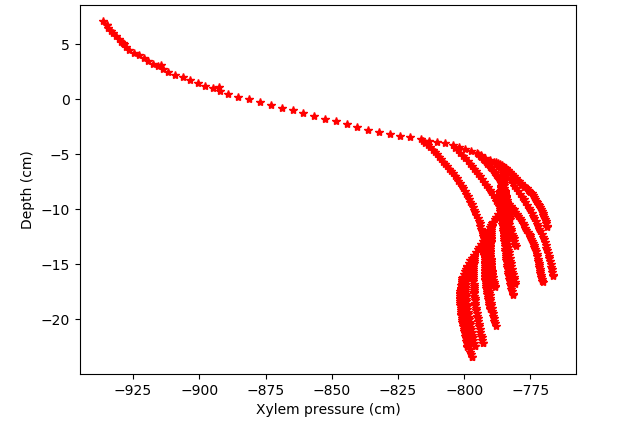
\includegraphics[width=0.99\textwidth]{example6e.png}
\subcaption{Calculated xylem matric potential (cm)} \label{fig:stomata}
\end{subfigure}
\begin{subfigure}[c]{0.5\textwidth}
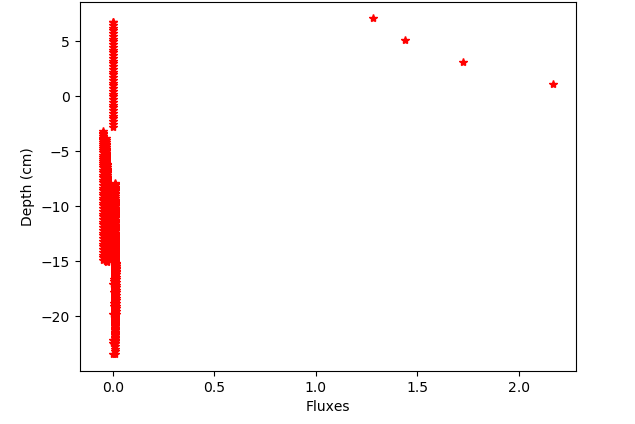
\includegraphics[width=0.99\textwidth]{example6e_2.png}
\subcaption{Radial water fluxes} \label{fig:stomatb}
\end{subfigure}
\caption{xylem potential and radial water fluxes per segment} 
\end{figure}

\subsubsection*{Coupling a static root system to DuMux} \label{sec:dumux_coupling}

Putting the sections \ref{ss:mapping} and \ref{ssec:xylem} together, we can easily set up an example, using the classic sink term in the soil model, similar as in \citep{leitner2014impact} based on \citep{doussan1998modelling}. For solving the Richards equation we use DuMux \citep{koch2020dumux}.

The next example mimics benchmark C12 \citep{schnepf2019call}, but with a static simulated root system. The example must be run out of dumux-rosi (located in dumux-rosi/rosi$\_$benchmarking/python$\_$solver/coupled), otherwise the DuMux Python coupling is not available. 

\lstinputlisting[firstline=1, language=Python, caption=Example 6c]{examples/example6c_coupling.py}

\begin{itemize}

\item[3,4] Add paths for DuMux Python coupling (L3) and Python solvers (L4).

\item[5,6] The direct C++ part of the DuMux binding, and the Python wrapper class. 

\item[17,18]  Defines a sinusoidal function for the collar boundary condition.

\item[21-37] All parameters that are needed for this simulation. L25 decides if periodic boundary conditions are used, or not. L35 states the simulation time, L36 the initial root system age. L37 defines if age dependent root conductivities are used. The rooot conductivities are hard coded in the file root\_conductivities.py, that is imported in L8. Age dependent conductities can be used to mimic root growth in a predefined way, i.e. the root system is already fully grown, but the radial conductivities are turned on during the simulation. 

\item[41-49] Sets up the soil solver (DuMux Python binding from dumux-rosi). 

\item[52-62] Sets up the Xylem model as in Subsection \ref{ssec:xylem}. If the root system is not periodic, a confining geometry is set L54-L58. L62 passes the axial and radial conductivities to the XylemFluxPython object (the function is defined in root\_conductivities.py).

\item[65-70] Coupling between the soil soil and root part is performed by setting the picking function that assigns a cell index to each spatial position L65, and L66. In L67 root segments are cut to the rectangular grid, and in L70 the cell index of the root collar is determined. 

\item[73-77] Initializes the simulation, initially the soil values are the same as the initial conditions (L75).

\item[79-94] First, we calculate the xylem matric potential $rx$ for a given soil matric potential $sx$ (L81) and save the actual collar flux for later analysis (L83). Next, we calculate teh sink (L85) and apply it to the soil model (L86). The soil model is simulated (L87) and the resulting matric potential $sx$ is updated (L88). The simulation takes some time (around 15 minutes), and L90-93 print debugging information and a progress bar. L94 increases the current simulation time. This is needed if age dependent conductivities are used. 

\item[99-111] L99 creates Figure \ref{fig:example6c} and, L102-111 plots uptake and cumulative uptake over time, see Figure \ref{fig:uptake}.

\end{itemize}

% \begin{figure}
% \begin{subfigure}[c]{0.5\textwidth}
% 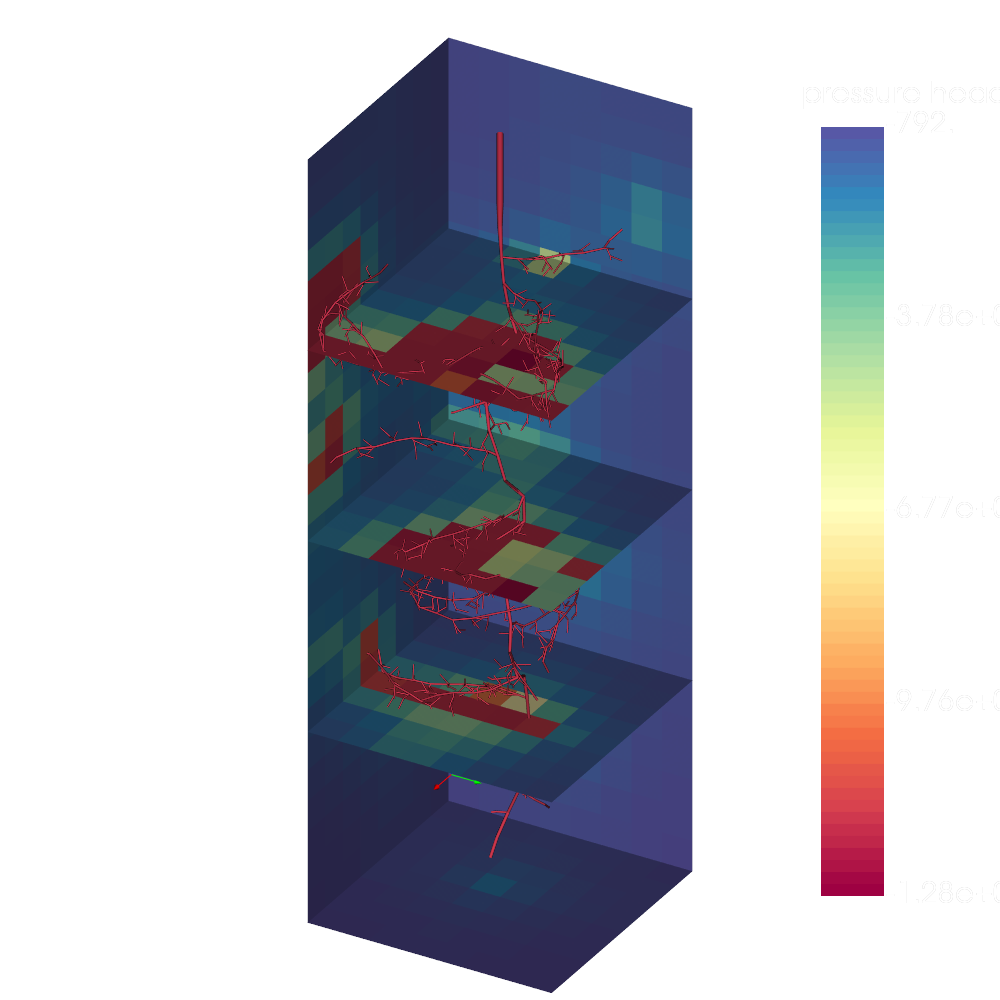
\includegraphics[width=0.99\textwidth]{example6c.png}
% \subcaption{Confined} \label{fig:example6c}
% \end{subfigure}
% \begin{subfigure}[c]{0.5\textwidth}
% 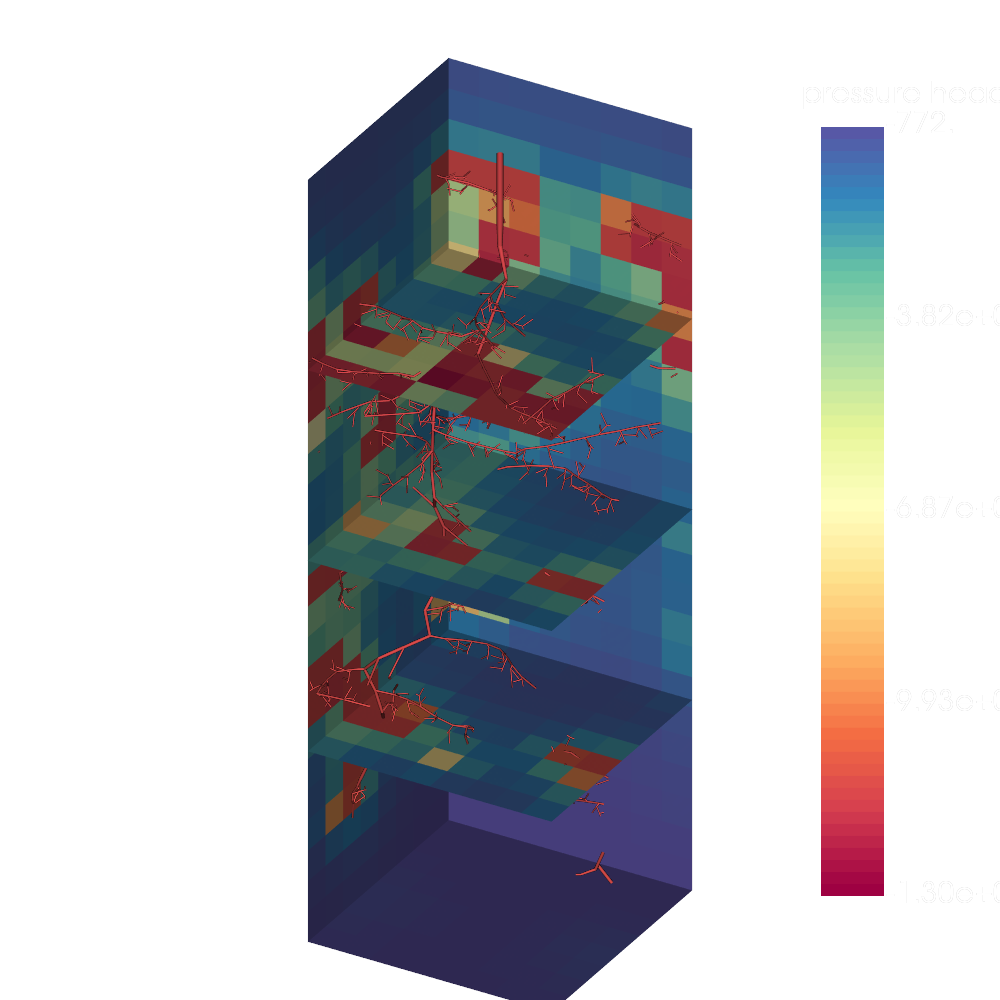
\includegraphics[width=0.99\textwidth]{example6c_periodic.png}
% \subcaption{Periodic boundary condtions} \label{fig:example6c_peridodic}
% \end{subfigure}
% \caption{Water depletion due to root uptake after one week. } \label{fig:example6c}
% \end{figure}

With above code we can compare total root system water uptake in a container, with the uptake if periodic boundary conditions are used. While the first scenario reflects the situation in a plant pot, periodic boundary conditions reflect the situation when the plant grows in the field, where the planting distance is approximately the domain size. Figure \ref{fig:uptake} shows both situations, showing that the boundary conditions will strongly affect total water uptake, because roots are less evenly distributed in the pot scenario and water redistribution is impeded by the pot boundaries.

% \begin{figure}
% \begin{subfigure}[c]{1\textwidth} 
% 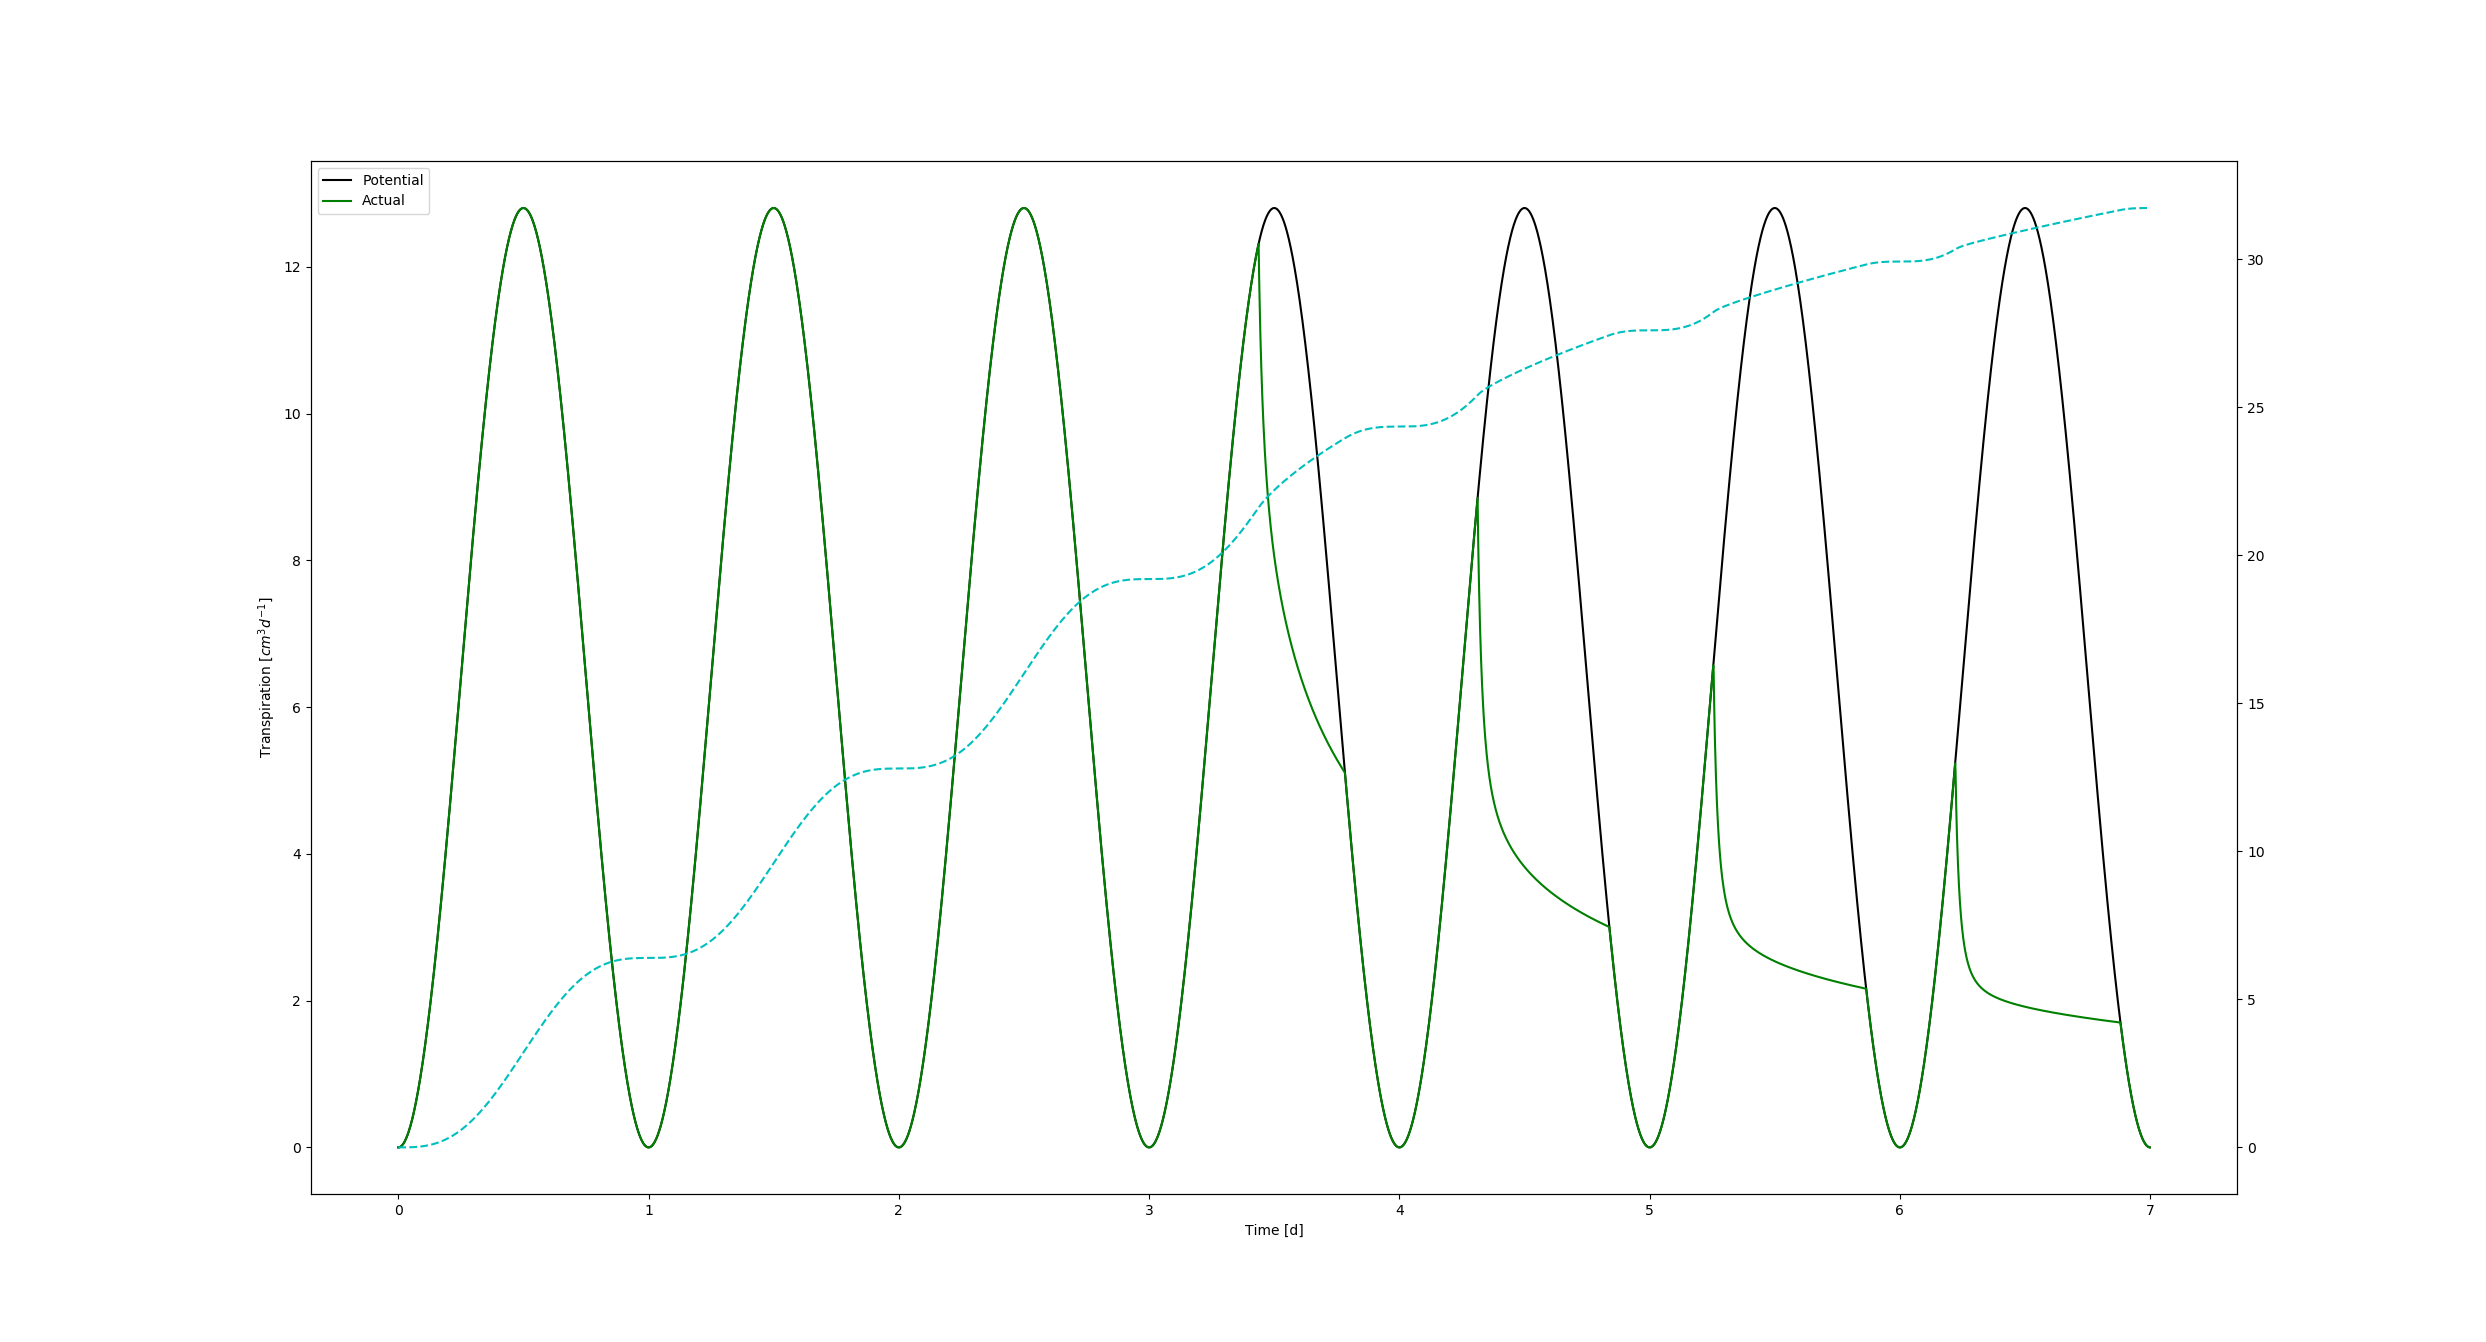
\includegraphics[width=0.99\textwidth]{Figure6c.png}
% \subcaption{Confined} \label{fig:uptake_confined}
% \end{subfigure}
% \begin{subfigure}[c]{1\textwidth}
% 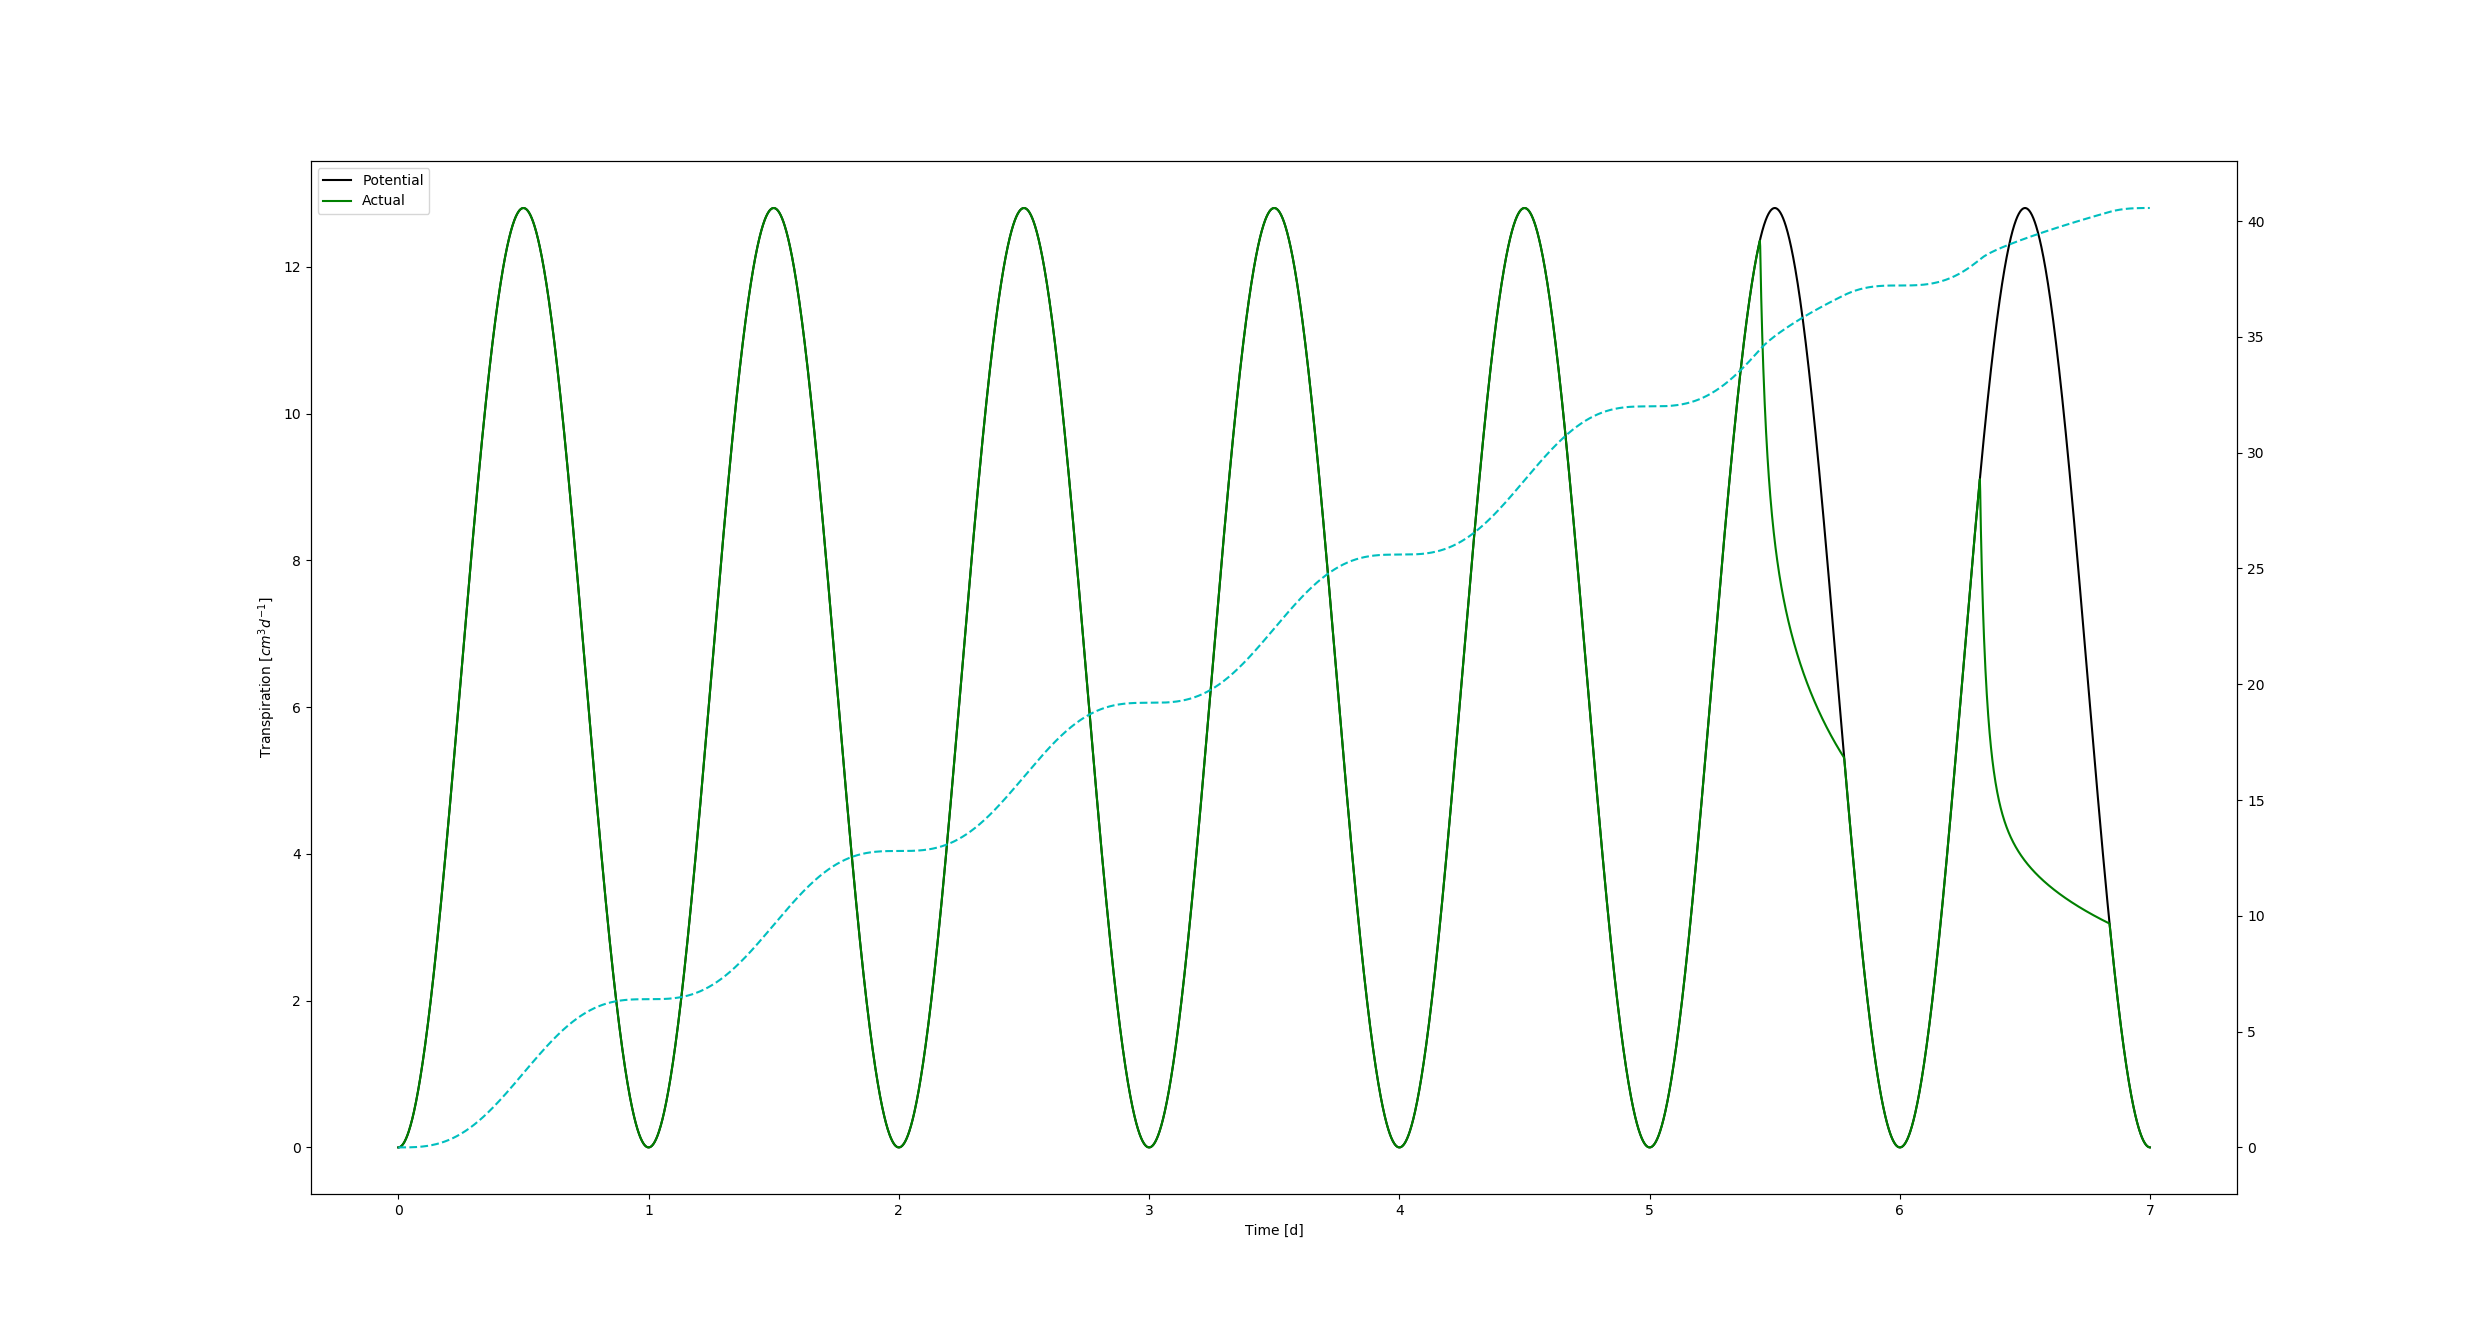
\includegraphics[width=0.99\textwidth]{Figure6c_periodic.png}
% \subcaption{Periodic boundary condtions} \label{fig:uptake_peridodic}
% \end{subfigure}
% \caption{Water uptake and cumulated uptake} \label{fig:uptake}
% \end{figure}
